\documentclass[11pt,titlepage]{article}
\usepackage{abstract}
\usepackage{changepage}
\usepackage[a4paper,headheight=15pt]{geometry}
\usepackage[myheadings]{fullpage}
\usepackage{fancyhdr}
\usepackage{lastpage}
\usepackage{url}
\usepackage[hidelinks,breaklinks]{hyperref}
\usepackage{breakurl}
\usepackage{xcolor}
\usepackage[numbers,sort]{natbib}
\usepackage[urw-garamond]{mathdesign}
\usepackage[T1]{fontenc}
\usepackage[font=small, labelfont=bf]{caption}
\usepackage[english]{babel}
\usepackage{sectsty}
\usepackage[nottoc,numbib]{tocbibind}
\usepackage{tocloft}
\usepackage{graphicx}
\usepackage{float}
\usepackage{pgfgantt}
\usepackage{textcomp}
\usepackage{epstopdf}

%-----------------------------------------------------------------
% CONFIG AND COMMANDS
%-----------------------------------------------------------------
\graphicspath{ {images/} }

\renewcommand*{\abstractnamefont}{
	\fontfamily{fos}
	\fontseries{b}
	\fontshape{sc}
	\selectfont
	\Large
}

\renewcommand{\cfttoctitlefont}{
	\fontfamily{fos}
	\fontseries{b}
	\fontshape{sc}
	\selectfont
	\Large
}

\renewcommand{\cftloftitlefont}{
	\fontfamily{fos}
	\fontseries{b}
	\fontshape{sc}
	\selectfont
	\Large
}

% Configure hyperlinks coloring.
\hypersetup{
	colorlinks,
	linkcolor={green!40!black},
	citecolor={blue!50!black},
	urlcolor={blue!80!black}
}

% Add new doi command that inserts url.
\newcommand*{\doi}[1]{\\\href{http://dx.doi.org/#1}{doi: #1}}

% Wide page for side by side figures, tables, etc.
\newlength{\offsetpage}
\setlength{\offsetpage}{1.0cm}
\newenvironment{widepage}{
	\begin{adjustwidth}{-\offsetpage}{-\offsetpage}%
    \addtolength{\textwidth}{2\offsetpage}}%
	{\end{adjustwidth}
}

\newcommand{\HRule}[1]{\rule{\linewidth}{#1}}

\renewcommand{\tocbibname}{References}

%-----------------------------------------------------------------
% HEADER & FOOTER
%-------------------------in----------------------------------------
\pagestyle{fancy}
\fancyhf{}
\fancyhead[L]{\small Agent Systems and Applications (Summer 2016)}
\fancyhead[R]{\small Report: Exercise 1}
\fancyfoot[R]{Page \thepage\ of \pageref{LastPage}}

\begin{document}

%-----------------------------------------------------------------
% TITLE
%-----------------------------------------------------------------
\title{ \normalsize \textsc{Agent Systems and Applications}
	\\ [2.0cm]
	\HRule{0.5pt} \\
	\fontfamily{fos}\fontseries{b}\fontshape{n}\selectfont
	\LARGE Report: Exercise 2
	\HRule{2pt} \\ [0.5cm]
	\normalsize \vspace{5\baselineskip}
	\normalfont \flushleft
	\textsc{Students:\\
		George, Sando\\
		Grinda, Constantin\\
		Lozano, David\\
		\vspace{2\baselineskip}
		Faculty of Mathematics and Information Science\\
		Warsaw University of Technology}\\
	\vspace{3\baselineskip}	
	\textsc{Guided By:\\
		prof. dr hab. Maria Ganzha (IBS PAN)\\
		prof. dr hab. Marcin Paprzycki (IBS PAN)}}


\author{}

\date{Summer 2016}
\maketitle

%\begin{abstract}

%\smallskip
%\noindent \textbf{Keywords.}
%\end{abstract}


\newpage
	\tableofcontents
	\listoffigures

%-----------------------------------------------------------------
% BODY
%-----------------------------------------------------------------
\sectionfont{\fontfamily{fos}\fontseries{b}\fontshape{sc}\selectfont}
\newpage
\section{Introduction}

Mobile agents are those agents that can migrate between networked systems in an effort to carry out a given task. This is a report on experiments conducted to test the performance of the agent mobility features of the JADE agent platform. The experiments were in the form of a simulated relay race between teams of mobile agents.


\section{Experiment Design}

\subsection{Scenario}

\begin{figure}[H]
	\begin{widepage}
		\centering
		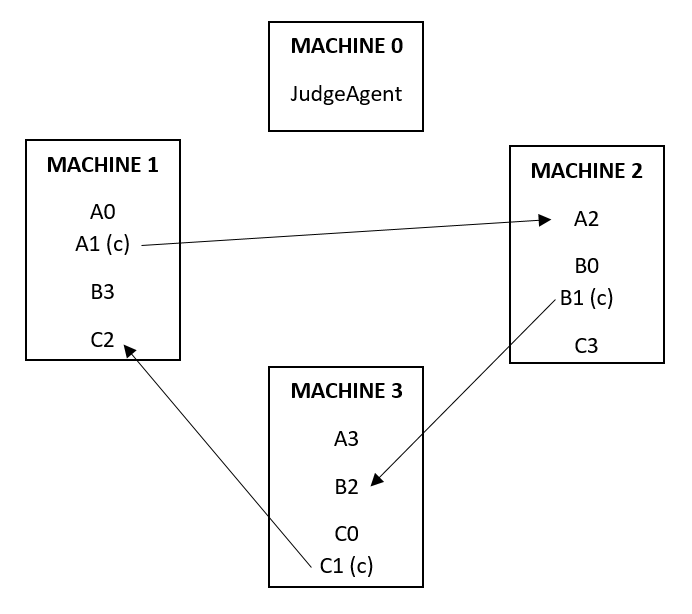
\includegraphics[width=0.5\textwidth]{scenario.png}
	\end{widepage}
	\caption{Sample scenario with 3 teams}
	\label{fig:Sample-scenario}
\end{figure}

The simulation is made up of teams of agents racing between containers located on different machines. To begin the simulation, a \emph{runner} agent from each team is placed on each machine. In addition to this, a captain \emph{runner} agent from each team is placed on each successive machine, so as to alternate the machines on which they begin the race.

To start the race, \emph{judge} agent sends a specific time to team captains. When it is the time, the captains moves from its container to the container of the next \emph{runner} agent on its team. Upon arriving at the next container, the \emph{runner} agent sends a message to its teammate on the container instructing it to move on to the next container. The previous \emph{runner} agent remains at its new location. When a given number of laps around the network is completed, the team signals to a \emph{judge} agent that it has completed the race. When all teams have completed the race, the \emph{judge} agent records the total time taken for all teams to complete the race.

The test parameters are varied as follows:

\begin{itemize}
	\item Increasing the number of machines gradually from 3 to 7.
	\item Varying the number of teams from 3 to 21.
	\item Varying the number of laps from 1 to 15.
\end{itemize}

\subsection{Machine Configuration}
The experiment was carried out on multiple Virtual Private Servers across the world from Linode VPS provider. 

The machines were deployed with the following configuration:

\begin{itemize}
	\item Compute: 1 CPU core
	\item Memory: 1024MB
	\item Storage: 24GB SSD
	\item Operating System: Ubuntu 14.04 LTS
	\item Linux Kernel Latest 64 bit (4.5.0\textendash x86\textunderscore 64\textendash linode65)
	\item Oracle Java 1.8
	\item JADE 4.4.0
\end{itemize}

\newpage
\section{Results}

The results obtained from the experiment are shown below.

\subsection{Number of Machines vs Runtime}

The number of machines was incresed gradually from 3 to 7 (without counting \emph{judge} agent's machine), with a fixed number of 3 teams and 10 laps.

\begin{figure}[H]
	\begin{widepage}
		\centering
		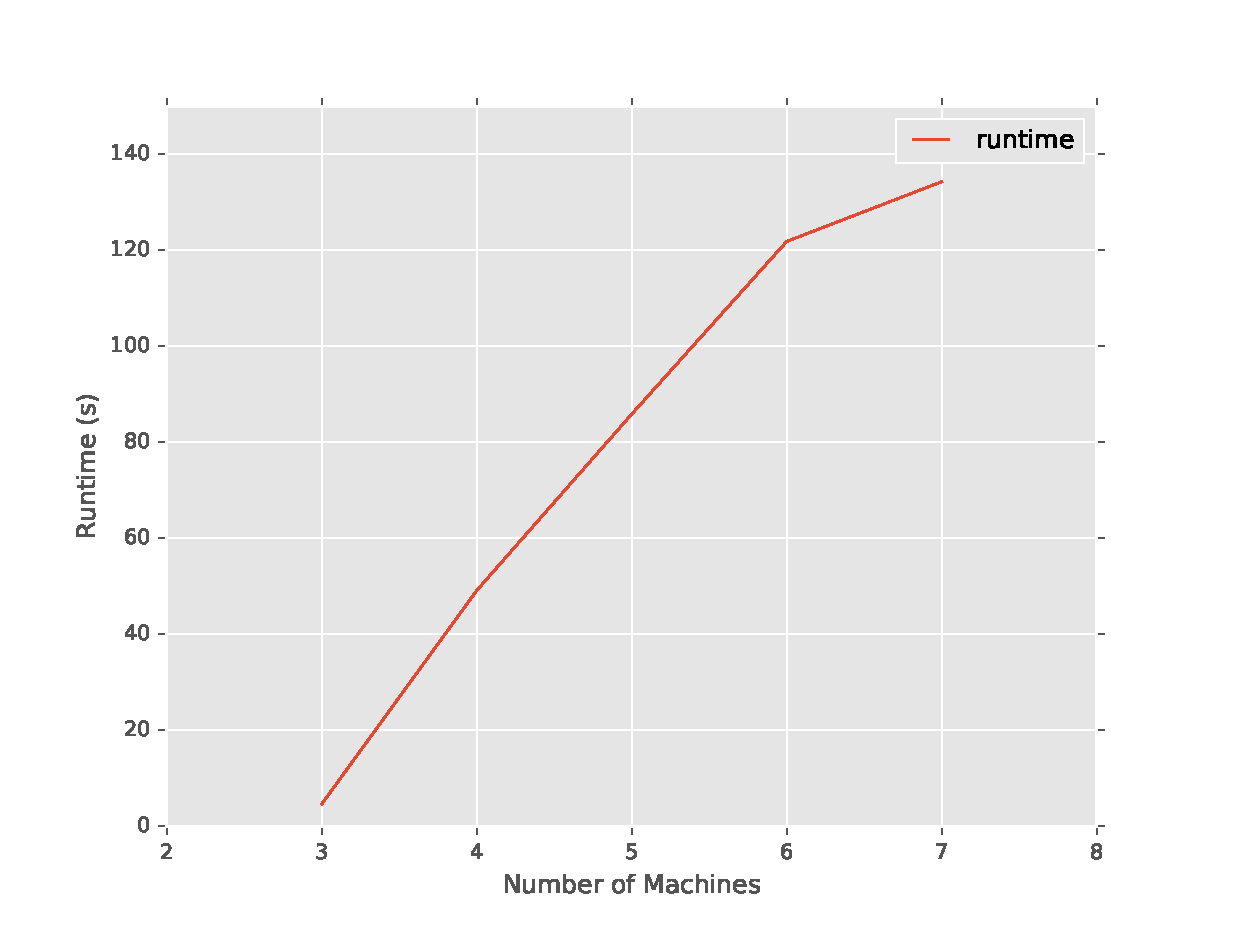
\includegraphics[width=0.5\textwidth]{machines.eps}
	\end{widepage}
	\caption{Num. Machines vs Runtime}
	\label{fig:Macs-Runtime}
\end{figure}

\subsection{Number of Teams vs Runtime}

The number of teams was increased gradually from 3 to 21, with a fixed number of 3 machines (without counting \emph{judge} agent's machine) and 10 laps.

\begin{figure}[H]
	\begin{widepage}
		\centering
		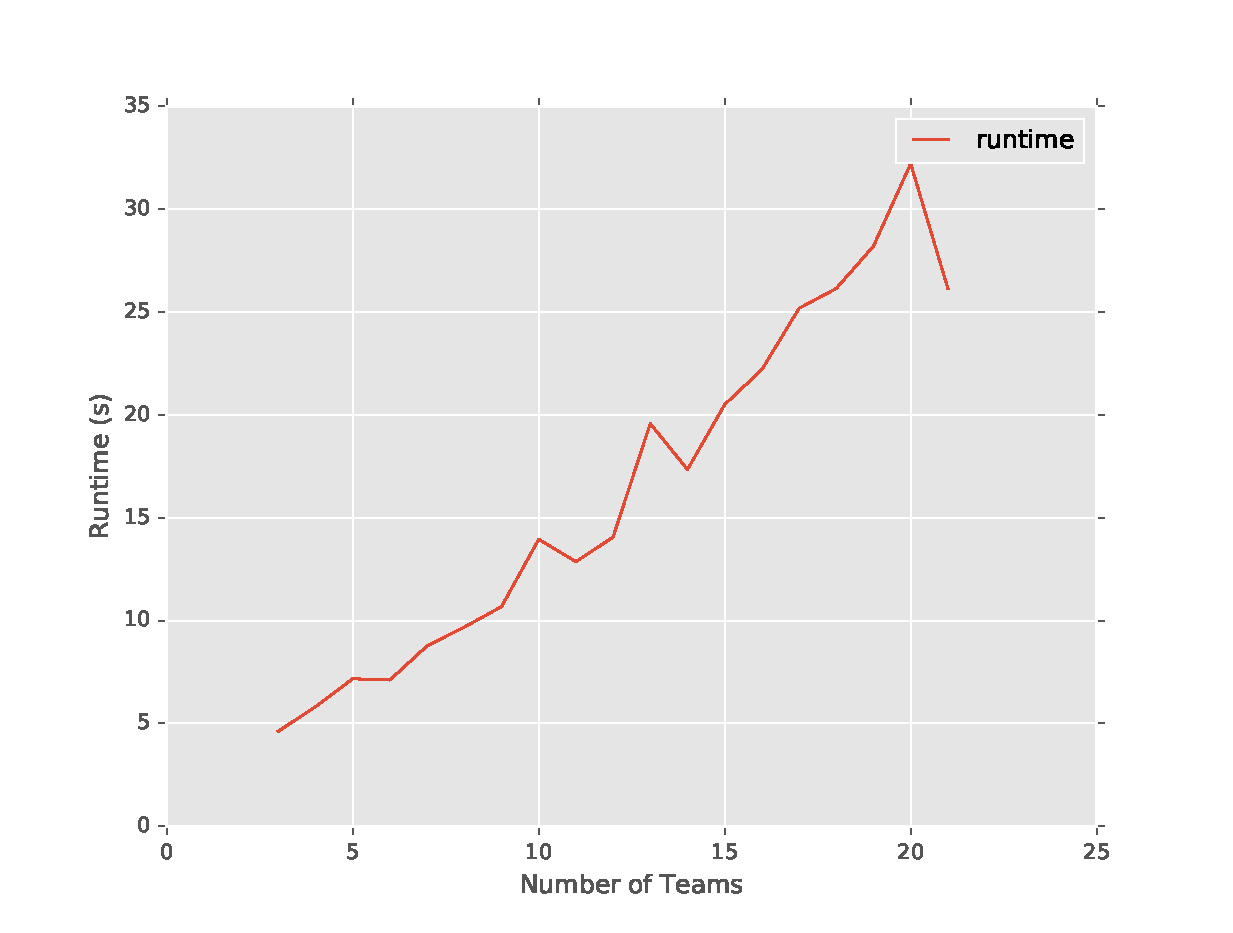
\includegraphics[width=0.5\textwidth]{teams.eps}
	\end{widepage}
	\caption{Num. Teams vs Runtime}
	\label{fig:Teams-Runtime}
\end{figure}

\subsection{Number of Laps vs Runtime}

The number of laps was increased gradually from 1 to 15, with a fixed number of 3 teams and 3 machines (without counting \emph{judge} agent's machine).

\begin{figure}[H]
	\begin{widepage}
		\centering
		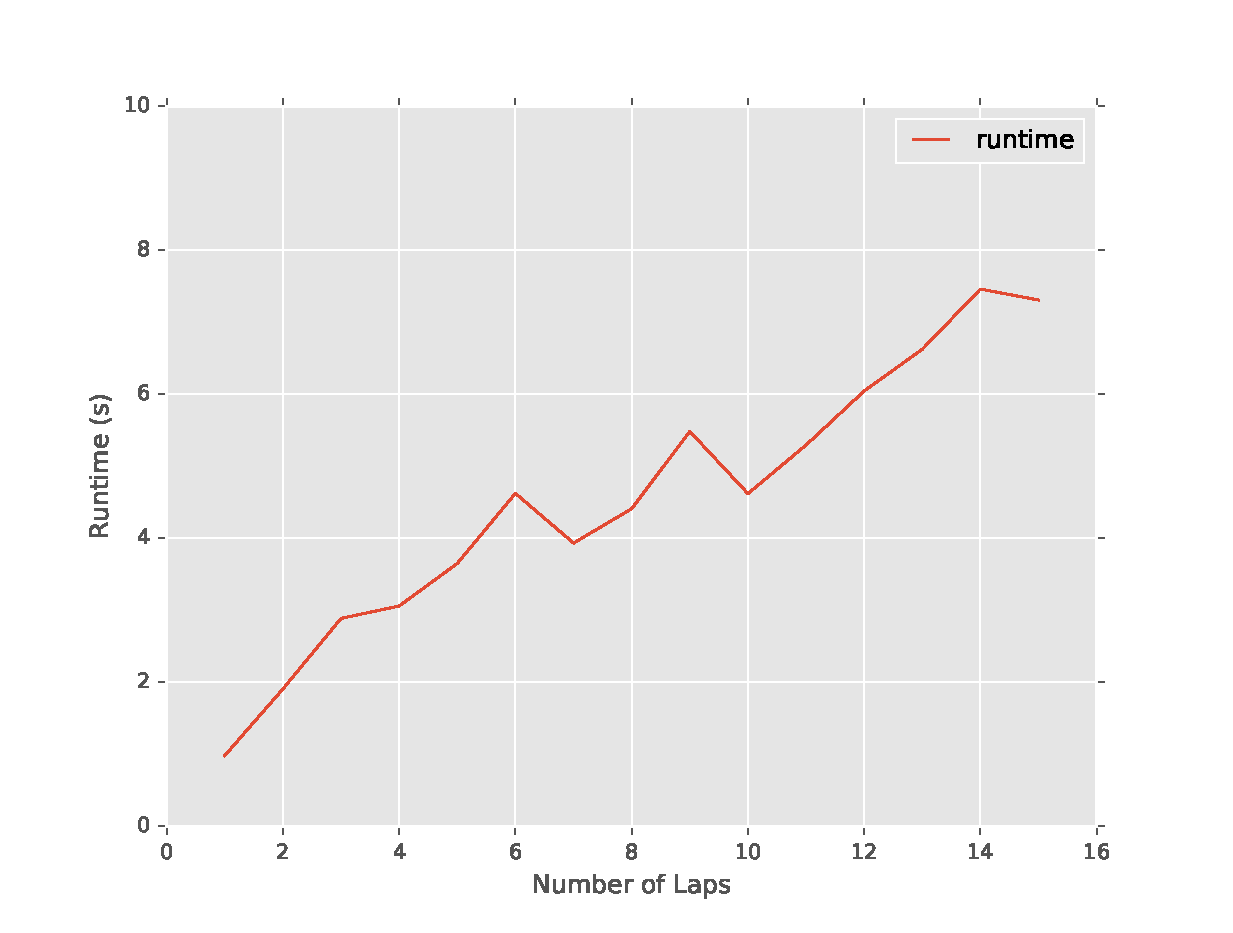
\includegraphics[width=0.5\textwidth]{laps.eps}
	\end{widepage}
	\caption{Num. Laps vs Runtime}
	\label{fig:Laps-Runtime}
\end{figure}

\section{Conclusion}

We can observe that, with small variation probably caused by network, there is a general trend of linearity in all the experiments, even with 21 teams of agents. We could then conclude that the performance of the mobility feature of the JADE agent platform scales in a linear manner. This should, therefore, be taken into consideration when designing systems, with JADE, that will employ agent mobility.

%\newpage
%\bibliography{citations}
%\bibliographystyle{plainnat}
\end{document}